
%(BEGIN_QUESTION)
% Copyright 2009, Tony R. Kuphaldt, released under the Creative Commons Attribution License (v 1.0)
% This means you may do almost anything with this work of mine, so long as you give me proper credit

Read and outline the ``Valve Sequencing Implementations'' subsection of the ``Split-Ranging'' section of the ``Control Valves'' chapter in your {\it Lessons In Industrial Instrumentation} textbook.  Note the page numbers where important illustrations, photographs, equations, tables, and other relevant details are found.  Prepare to thoughtfully discuss with your instructor and classmates the concepts and examples explored in this reading.

\underbar{file i04209}
%(END_QUESTION)





%(BEGIN_ANSWER)


%(END_ANSWER)





%(BEGIN_NOTES)

Alternative options for split-ranging two control valves:

\begin{itemize}
\item{} Single I/P with two valves of differing bench-sets 
\item{} Dual I/P converters 
\begin{itemize}

\item{} Sequencing done in I/Ps (differing I/P calibrations)
\end{itemize}
\item{} Dual controller outputs (e.g. DCS or PLC) 
\begin{itemize}

\item{} Sequencing done in I/Ps (differing I/P calibrations)
\item{} Sequencing done in controller (or ``SPLT'' function block in FF)
\end{itemize}
\item{} Dual controllers 
\begin{itemize}

\end{itemize}
\end{itemize}

\vskip 10pt

The location of the sequencing affects fail-safe modes for both valves.  For example, complementary or exclusive split-ranged valves controlled by a common signal from a controller will fail in opposite directions if that common signal fails.  However, we may achieve the same kind of sequencing using dual outputs from the controller, with split-ranging done inside the controller, and enjoy valves with common fail-safe modes.











\vskip 20pt \vbox{\hrule \hbox{\strut \vrule{} {\bf Suggestions for Socratic discussion} \vrule} \hrule}

\begin{itemize}
\item{} Explain how split-ranging may be done in two different ways for the reactor heating/cooling control system shown in this section.
\item{} Explain why the fail-safe modes are not the same between the two different reactor heating/cooling control systems.
\item{} Examine the FOUNDATION Fieldbus function block diagram examples and explain what they represent and where an engineer or technician may access them to change their connections or parameters.
\item{} Examine the page in the textbook showing four different methods of split-ranging, and assume the split-ranging in each case is {\it complementary}.  Then, ask students to calculate the positions of the two control valves given some arbitrary output signal from the controller.
\item{} Examine the page in the textbook showing four different methods of split-ranging, and assume the split-ranging in each case is {\it complementary}.  Then, pose a fault in one of those systems and ask students to identify the consequence(s) of that fault on the positions of both control valves.  Where applicable, ask students to explain how the same fault would manifest in different consequences for each of the split-ranging methods shown.
\end{itemize}







\vfil \eject

\noindent
{\bf Summary Quiz:}

A pair of progressively-sequenced control valves send cooling water to a chemical reaction vessel:

$$\includegraphics[width=15.5cm]{i04209x01.eps}$$

Suppose an operator leaves the controller for this loop in manual mode, with the output fixed at 8 milliamps.  Determine the positions of the two control valves:

\begin{itemize}
\item{} Valve A 75\% open; Valve B 25\% open
\vskip 5pt 
\item{} Both valves fully shut
\vskip 5pt 
\item{} Valve A 25\% open; Valve B 75\% open
\vskip 5pt 
\item{} Valve A fully shut; Valve B 50\% open
\vskip 5pt 
\item{} Both valves 100\% open
\vskip 5pt 
\item{} Valve A 50\% open; Valve B fully shut
\end{itemize}



%INDEX% Reading assignment: Lessons In Industrial Instrumentation, split-ranging (implementations)

%(END_NOTES)


